% =============================================================================
% COPYRIGHT AND DISCLAIMER
% =============================================================================
% This file is provided as a convenience template for competition participants.
% By using it, you accept full responsibility for compliance with all applicable
% copyright, licensing, and usage rules of the Association for Computing
% Machinery (ACM) and of any LaTeX packages you load (including, without
% limitation, the "acmart" document class and related ACM materials).
%
% Consult ACM's official publication, template, and copyright policies before
% using this setup for any purpose other than this competition. Do not assume
% that this template may be reused, redistributed, or submitted elsewhere
% without independently verifying ACM's current rules.
%
% Use of the "acmart" class, the "sigconf" option, or ACM-style formatting in
% this template does NOT mean that this report, this competition, its organizers,
% or any resulting PDF is sponsored, endorsed, affiliated with, or published by
% ACM. ACM trademarks and branding remain the property of ACM.
%
% Template packages live in preamble.tex.
% Citations live in main.bib. Edit this file with your paper content.
% =============================================================================

\documentclass[sigconf]{acmart}
% =============================================================================
% Template setup — participants normally do not edit this file.
% Author content belongs in main.tex; citations belong in main.bib.
% \documentclass lives in main.tex so Overleaf does not treat this file as root.
% =============================================================================

% --- Competition / non-ACM-submission friendly rights metadata -------------
\setcopyright{none}
\settopmatter{printacmref=false}
\acmConference[Kaggle Competition]{Filament Segmentation Challenge}{2026}{\href{https://www.kaggle.com/competitions/filament-segmentation-2026}{kaggle.com/competitions/filament-segmentation-2026}}
\acmBooktitle{Competition Report}
\acmDOI{}
\acmISBN{}

% --- Author guidance text --------------------------------------------------
% \guide{...} is gray italic while \guideStyletrue; omitted from the PDF if false.
% Flip the switch in main.tex after % =============================================================================
% Template setup — participants normally do not edit this file.
% Author content belongs in main.tex; citations belong in main.bib.
% \documentclass lives in main.tex so Overleaf does not treat this file as root.
% =============================================================================

% --- Competition / non-ACM-submission friendly rights metadata -------------
\setcopyright{none}
\settopmatter{printacmref=false}
\acmConference[Kaggle Competition]{Filament Segmentation Challenge}{2026}{\href{https://www.kaggle.com/competitions/filament-segmentation-2026}{kaggle.com/competitions/filament-segmentation-2026}}
\acmBooktitle{Competition Report}
\acmDOI{}
\acmISBN{}

% --- Author guidance text --------------------------------------------------
% \guide{...} is gray italic while \guideStyletrue; omitted from the PDF if false.
% Flip the switch in main.tex after % =============================================================================
% Template setup — participants normally do not edit this file.
% Author content belongs in main.tex; citations belong in main.bib.
% \documentclass lives in main.tex so Overleaf does not treat this file as root.
% =============================================================================

% --- Competition / non-ACM-submission friendly rights metadata -------------
\setcopyright{none}
\settopmatter{printacmref=false}
\acmConference[Kaggle Competition]{Filament Segmentation Challenge}{2026}{\href{https://www.kaggle.com/competitions/filament-segmentation-2026}{kaggle.com/competitions/filament-segmentation-2026}}
\acmBooktitle{Competition Report}
\acmDOI{}
\acmISBN{}

% --- Author guidance text --------------------------------------------------
% \guide{...} is gray italic while \guideStyletrue; omitted from the PDF if false.
% Flip the switch in main.tex after \input{preamble}.
%
% Do not use \guide{...} for \email{...}.
\usepackage{xcolor}
\newif\ifguideStyle
\guideStyletrue
\newcommand{\guide}[1]{%
  \ifguideStyle
    {\color{gray!65}\itshape #1}%
  \fi
}

% --- Math ------------------------------------------------------------------
% Do NOT load amssymb (or amsfonts): acmart already loads newtxmath, which
% defines the same symbols (e.g. \Bbbk) and causes a conflict on Overleaf.
% amsmath is already provided by acmart; mathtools extends it.
\usepackage{mathtools}

% --- Figures ---------------------------------------------------------------
% graphicx is already loaded by acmart
\usepackage{subcaption}

% --- Tables ----------------------------------------------------------------
% booktabs is already loaded by acmart
\usepackage{tabularx}
\usepackage{multirow}

% --- Bibliography style is set in main.tex (ACM-Reference-Format) ----------
.
%
% Do not use \guide{...} for \email{...}.
\usepackage{xcolor}
\newif\ifguideStyle
\guideStyletrue
\newcommand{\guide}[1]{%
  \ifguideStyle
    {\color{gray!65}\itshape #1}%
  \fi
}

% --- Math ------------------------------------------------------------------
% Do NOT load amssymb (or amsfonts): acmart already loads newtxmath, which
% defines the same symbols (e.g. \Bbbk) and causes a conflict on Overleaf.
% amsmath is already provided by acmart; mathtools extends it.
\usepackage{mathtools}

% --- Figures ---------------------------------------------------------------
% graphicx is already loaded by acmart
\usepackage{subcaption}

% --- Tables ----------------------------------------------------------------
% booktabs is already loaded by acmart
\usepackage{tabularx}
\usepackage{multirow}

% --- Bibliography style is set in main.tex (ACM-Reference-Format) ----------
.
%
% Do not use \guide{...} for \email{...}.
\usepackage{xcolor}
\newif\ifguideStyle
\guideStyletrue
\newcommand{\guide}[1]{%
  \ifguideStyle
    {\color{gray!65}\itshape #1}%
  \fi
}

% --- Math ------------------------------------------------------------------
% Do NOT load amssymb (or amsfonts): acmart already loads newtxmath, which
% defines the same symbols (e.g. \Bbbk) and causes a conflict on Overleaf.
% amsmath is already provided by acmart; mathtools extends it.
\usepackage{mathtools}

% --- Figures ---------------------------------------------------------------
% graphicx is already loaded by acmart
\usepackage{subcaption}

% --- Tables ----------------------------------------------------------------
% booktabs is already loaded by acmart
\usepackage{tabularx}
\usepackage{multirow}

% --- Bibliography style is set in main.tex (ACM-Reference-Format) ----------


% Guide styling: \guideStyletrue = show gray italic hints; \guideStylefalse = omit them
% DRAFT: kept on so that the author placeholders below stay visible; switch to \guideStylefalse when they are filled in.
\guideStyletrue
% \guideStylefalse

\begin{document}

\title{A Learned Candidate Scorer over Two Mask2Former Families for Solar Filament Instance Segmentation}
\subtitle{A Solution to the Solar Filament Segmentation Challenge 2026} % DO NOT CHANGE


\author{\guide{Firstname Lastname}}  % TODO: author name
\affiliation{%
  \institution{\guide{Your Institution}}  % TODO: or remove
  \city{\guide{City}}
  \country{\guide{Country}}
}
\email{first.author@example.com}   % TODO: your email

\begin{abstract}
    This report describes our solution to the Solar Filament Segmentation Challenge~2026, a Kaggle competition on automatic segmentation of solar filaments in GONG H-$\alpha$ observations. Our candidate filaments come from two Mask2Former families trained at native resolution on 5 date-grouped folds, one reading the photograph and one reading a limb-darkening-corrected version of it. Their 16 test-time views are fused into one pool of candidates per image. Most annotated filaments already have a matching candidate among them (85--89\% in our first model's pool), so the main difficulty is choosing which candidates to submit. A gradient-boosted scorer predicts, for each candidate, the IoU it is expected to reach with the annotators' filaments, from 76 numbers that include its agreement with independently trained detectors and U-Nets. An exact integer program then keeps the non-overlapping set that maximises the expected gain in panoptic quality, and the boundary of each kept mask is redrawn from full-resolution U-Net maps. On 5-fold cross-validation over all 707 training observations, the pipeline reaches a panoptic quality (PQ) of 0.4770 (95\% bootstrap interval 0.4685--0.4854), against 0.4629 for one Mask2Former family with a fixed score threshold.
\end{abstract}

\maketitle

\ifguideStyle
\noindent{\color{gray!65}\itshape
Guide mode is on.}
\par\medskip
\fi


% ==================================== %
%              INTRODUCTION            %
% ==================================== %
\section{Introduction}
    This report goes over the details of our submitted solution to the Solar Filament Segmentation Challenge~2026 \cite{filament-segmentation-2026}. The challenge, launched on July~10,~2026, is organized by the Earth-Space AI Research (ESAIR) Lab\footnote{\href{https://www.esairlab.com/home}{www.esairlab.com/}}. This challenge utilizes the MAGFiLO dataset for evaluation of the segmentation algorithms \cite{ahmadzadeh2024dataset}. Each filament must be returned as its own mask, and a mask only counts when its IoU with an annotated filament is above 0.5, for each annotator of the image separately.

    Two observations shaped our solution. First, candidate generation is not the bottleneck: the 8-view candidate pool of our first model already held a matching candidate for 85--89\% of the annotated filaments, while a fixed score threshold submitted only about two thirds of them. Second, the annotations are noisy: scored against each other, two annotators of the same image reach a PQ of only 0.340. We therefore spent most of our effort on deciding which candidates to submit, with a scorer trained on the exact question the metric asks, and checked every step on out-of-fold PQ with paired bootstrap intervals. Our code, the trained models and a notebook that rebuilds the submitted file byte for byte are available in our repository; parts of the code are adapted from open-source projects, credited in its \texttt{THIRD\_PARTY\_NOTICES.md}.


% ==================================== %
%              METHODOLOGY             %
% ==================================== %
\section{Methodology}\label{sec:methodology}

\begin{figure*}[t]
\centering
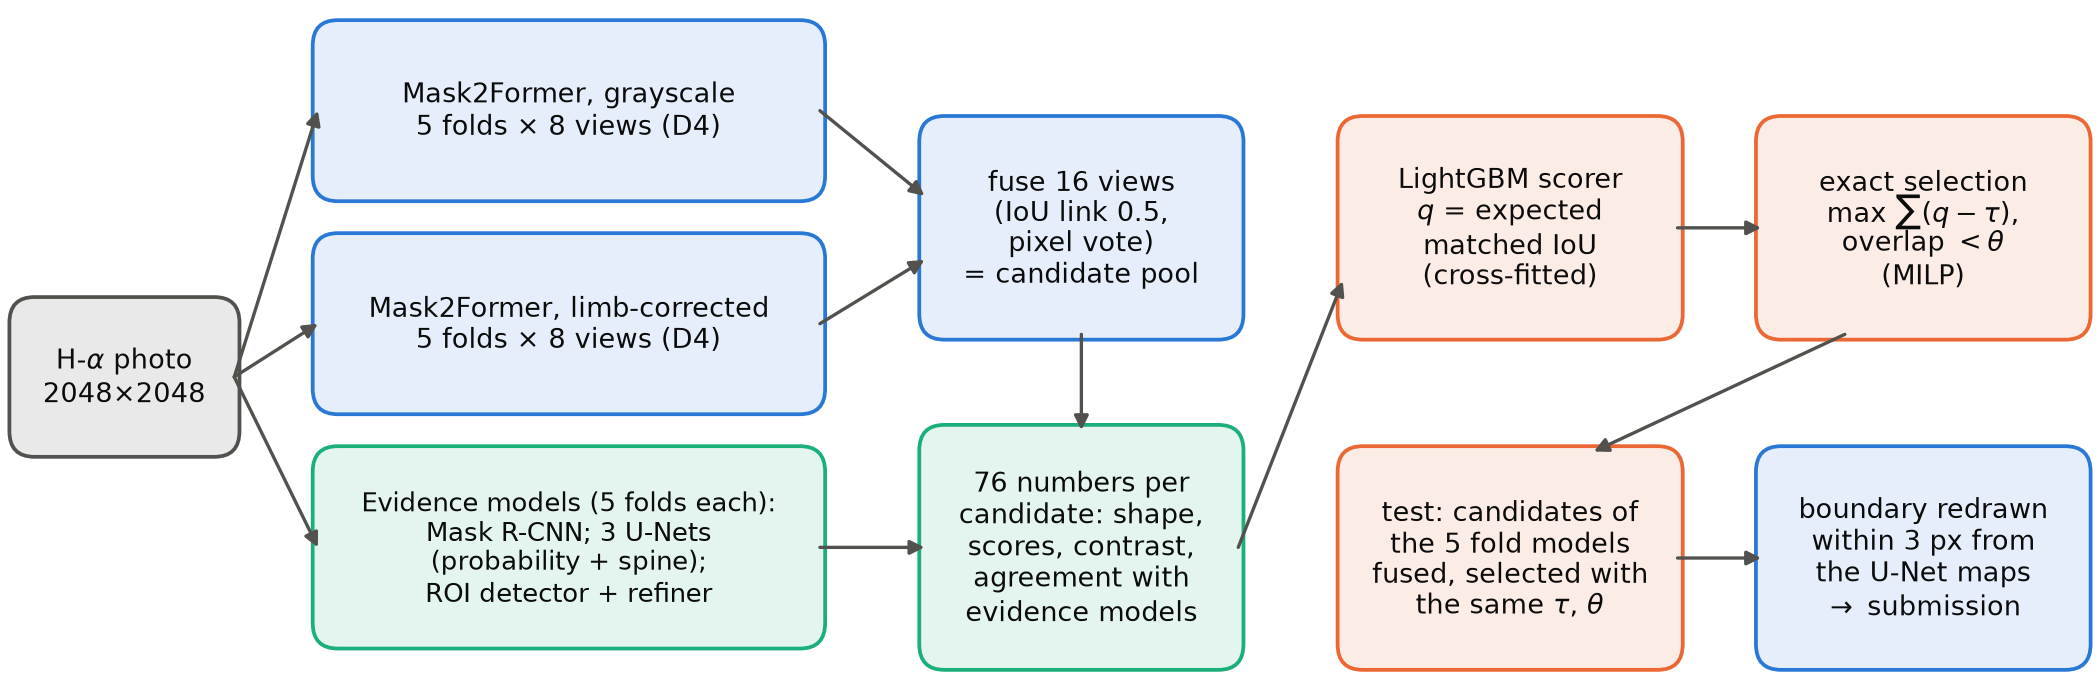
\includegraphics[width=\textwidth]{figures/pipeline.png}
\caption{The pipeline. Every model family is trained 5 times, once per fold. On a training photograph, every number comes from models that did not train on its fold; on a test photograph, the candidates of the 5 fold models are fused before the selection.}
\label{fig:pipeline}
\Description{Flow chart: the photograph feeds two Mask2Former families and three kinds of evidence models; the 16 Mask2Former views are fused into a candidate pool; 76 numbers per candidate feed a LightGBM scorer; an exact selection, a 5-fold fusion on test and a boundary redraw produce the submission.}
\end{figure*}

Fig.~\ref{fig:pipeline} shows the whole pipeline.

\subsection{Data and sampling}
The training set has 707 GONG \cite{harvey1996gong} observations: 411 were annotated by one annotator, 145 by two and 151 by three, giving 1,154 annotator records with about 8,200 filaments. A filament persists on the disk for days, so we split the observations into 5 folds grouped by date. Every model family is trained 5 times, model $k$ on the observations of the other four folds; its predictions on fold $k$ are therefore out of fold (OOF), and every training observation is predicted by models that never saw it. The second-level scorer is cross-fitted on the same folds. On test, the 5 fold models of each family all predict.

\subsection{Candidate generation: two Mask2Former families}
Both families are Mask2Former \cite{cheng2022mask2former} with a Swin-S backbone \cite{liu2021swin}, started from COCO \cite{lin2014coco} instance-segmentation weights. They train for 50 epochs at native resolution, on 1024-pixel crops and on whole 2048-pixel frames, with a batch of 8 obtained by gradient accumulation, bf16 and the loss of the reference implementation. One sample is one annotator record. On a 12\,GB GPU one fold trains in about 5.5 hours. The first family reads the grayscale photograph. The second reads three channels: the photograph, the solar disk divided by its radial median profile (a limb-darkening correction that is robust to the filaments themselves; the disk is found by a Hough circle on the limb), and a CLAHE \cite{zuiderveld1994clahe} copy of that flattened disk; its training crops are also zoomed by a random factor in $[0.8, 1.25]$. Alone, the second family is not better (OOF single-view PQ 0.4606 against 0.4630, mean over folds); fused with the first, it adds about 25\% candidates to each pool, but little to the final score (Section~\ref{sec:evaluation}).

The mask logits are predicted at a quarter of the input resolution, upsampled bilinearly to 2048 pixels and thresholded at zero; a candidate's score is its class probability times its mean mask probability, and every query above a score of 0.02 becomes a candidate. Each fold model predicts the 8 rotations and reflections of the image. The 16 views of a fold's two models are fused: candidates whose IoU exceeds 0.5 are linked, a group's mask is the pixel-wise majority of its members, and its score is the mean member score times $(0.5 + 0.5\,m/16)$ for a group of $m$ members.

\subsection{Evidence models}
Three kinds of models, trained on the same folds, check each candidate independently. A Mask R-CNN \cite{he2017maskrcnn} (ResNet-50 FPN v2, COCO start, 1024-pixel crops, 12k iterations) proposes its own instances. Three U-Nets \cite{ronneberger2015unet}, with ConvNeXt-T \cite{liu2022convnext} encoders trained for 24k and 48k steps and a ResNet-34 \cite{he2016resnet} encoder trained for 30k steps, predict two full-resolution maps: the filament probability (target: the fraction of annotators who marked the pixel) and the filament spine (its centre line); the loss is BCE plus 0.5 Dice on the first map plus 0.3 BCE on the second. A tiled detector (Faster R-CNN v2 \cite{ren2015faster} on 9 tiles of the disk) with a ResNet-18 U-Net that redraws the mask inside each box's context crop gives a third, region-based set of instances.

\subsection{A scorer trained on the metric's question}
For each candidate of a training observation, the target is the mean over the observation's annotator records of the IoU between the candidate and the annotated filament it overlaps most, counted as zero when this IoU is not above 0.5; this is exactly what the candidate adds to the PQ numerator, per record. The scorer sees 76 numbers per candidate. Thirty describe the candidate itself: its fused score, its agreement with the single-view predictions, its area, box and elongation, its distance from the disk centre, the intensity and contrast of the photograph inside and around it, and its competitors (the overlapping candidates and their scores). The other 46 describe what the evidence models say about it: its best IoU with a Mask R-CNN instance and that instance's score (5 numbers), the same for the tiled detector (5), and for each U-Net the spine map inside and around the mask and how the mask covers the map's own connected regions (12 each). The scorer is LightGBM \cite{ke2017lightgbm} (regression, 300 rounds, 15 leaves, learning rate 0.05), averaged over 5 seeds and weighted by the number of records. Its OOF predictions correlate with the target at 0.778; the candidates' own fused score correlates at 0.702.

\subsection{Exact selection, test fusion and boundary redraw}
For PQ $= \sum_{\mathrm{TP}} \mathrm{IoU} \,/\, (|\mathrm{TP}| + \tfrac12 |\mathrm{FP}| + \tfrac12 |\mathrm{FN}|)$ \cite{kirillov2019panoptic}, adding a non-overlapping mask raises the score only if its expected matched IoU exceeds PQ/2. Among a photograph's candidates we therefore keep the set that maximises $\sum (q - \tau)$, where $q$ is the scorer's prediction, subject to no two kept masks overlapping by more than a fraction $\theta$ of the smaller one. Candidates with $q \le \tau$ are dropped, the conflict graph of the others splits into connected components, and each component is solved exactly as a 0/1 integer program with HiGHS \cite{huangfu2018highs}. The kept masks are painted in decreasing $q$, so that each pixel goes to one mask, and masks under 100 pixels are dropped. A grid over the OOF observations gives $\tau = 0.225$ and $\theta = 0.1$; $\tau$ is close to PQ/2, as expected.

On test, the scorer is retrained on all OOF rows. The candidates of the 5 fold models are fused (IoU link 0.5, pixel vote), a group's $q$ is the mean over the 5 models of that model's best member (zero for a model without one), and the same $\tau$ and $\theta$ select the instances; nothing is tuned on test.

Mask2Former's masks come from quarter-resolution logits, while the U-Nets predict at full resolution. Each kept mask $M$ therefore keeps its extent, and its boundary is redrawn within $r$ pixels from $P$, the mean of the two U-Nets' probability maps: $M' = \mathrm{erode}(M, r) \cup \big((P > t) \cap \mathrm{dilate}(M, r)\big)$, with the threshold $t$ chosen per mask to best reproduce $M$. Out of fold, $r = 1$ and $r = 3$ pixels are equivalent (0.4774 against 0.4770, difference $-0.0003$, 95\% interval $-0.0012$ to $+0.0006$); the final submission uses $r = 3$.


% ==================================== %
%              EVALUATION              %
% ==================================== %
\section{Evaluation}\label{sec:evaluation}

\subsection{Strategy}
All numbers are OOF PQ over the 707 training observations: each annotator record is matched separately, true positives, false positives and false negatives are pooled over all records, and PQ is computed once, as in the competition's scorer. Every choice (model families, epochs, scorer settings, $\tau$, $\theta$) was made on this OOF PQ. A difference between two variants is judged with a paired bootstrap over observations (4,000 resamples, the same observations in both arms); the uncertainty of a single score with an unpaired bootstrap (5,000 resamples). To check that the threshold choice is not overfitted, $\tau$ is also chosen on 4 folds and applied to the fifth (nested).

\subsection{Results}
Table~\ref{tab:results} adds one step at a time on the same observations. The learned scorer is the largest single gain, and it needs the evidence models: on candidate numbers alone it does no better than a fixed threshold on the same pool (0.4693 against 0.4693, difference $0.0000$, 95\% interval $-0.0027$ to $+0.0027$). Table~\ref{tab:evidence} adds the evidence blocks one at a time: the U-Net spine maps bring most of the gain, while the tiled detector adds nothing measurable. The second Mask2Former family adds little as well: the same pipeline on the grayscale family alone scores 0.4766, a difference of $-0.0004$ (95\% interval $-0.0028$ to $+0.0020$). The final pipeline scores 0.4770 (bootstrap standard deviation 0.0043, 95\% interval 0.4685--0.4854). Its five folds score 0.4747, 0.4870, 0.4703, 0.4800 and 0.4732 (standard deviation 0.0066), so differences below about 0.004 between single rows are within noise; the paired intervals of Table~\ref{tab:results} are narrower because both arms share the same observations. The final pipeline submits 7,766 masks against the 8,199 annotated ones (counted per record): 5,517 are matched, with a mean IoU of 0.690. Fig.~\ref{fig:examples} shows OOF predictions and Fig.~\ref{fig:redraw} the boundary redraw.

\begin{table}[t]
\centering
\small
\caption{OOF PQ on the 707 training observations, adding one step at a time. $\Delta$: paired difference with the row above (last row: with the final pipeline), with its 95\% bootstrap interval.}
\label{tab:results}
\begin{tabular}{lcc}
\toprule
Step & OOF PQ & $\Delta$ [95\% interval] \\
\midrule
Grayscale family, single view, score $>0.85$ & 0.4629 & -- \\
Two families, 16-view pool, score $>0.75$ & 0.4693 & -- \\
+ learned scorer, exact selection (nested $\tau$) & 0.4739 & $+0.0046$ [$+0.0014$, $+0.0076$] \\
\quad $\tau$ chosen on all folds & 0.4750 & -- \\
+ boundary redraw, $r=3$ & 0.4770 & $+0.0021$ [$+0.0007$, $+0.0035$] \\
\midrule
Same pipeline, grayscale family only & 0.4766 & $-0.0004$ [$-0.0028$, $+0.0020$] \\
\bottomrule
\end{tabular}
\end{table}

\begin{table}[t]
\centering
\small
\caption{Evidence blocks of the scorer (OOF PQ as emitted, $\tau$ chosen on 4 folds and applied to the fifth). Correlation: OOF prediction against the target.}
\label{tab:evidence}
\begin{tabular}{lccc}
\toprule
Scorer inputs & Numbers & Correlation & OOF PQ \\
\midrule
Candidate only & 30 & 0.772 & 0.4693 \\
+ Mask R-CNN & 35 & 0.776 & 0.4712 \\
+ 3 U-Net spine maps & 71 & 0.777 & 0.4745 \\
+ tiled detector & 76 & 0.778 & 0.4739 \\
\bottomrule
\end{tabular}
\end{table}

\begin{figure*}[t]
\centering
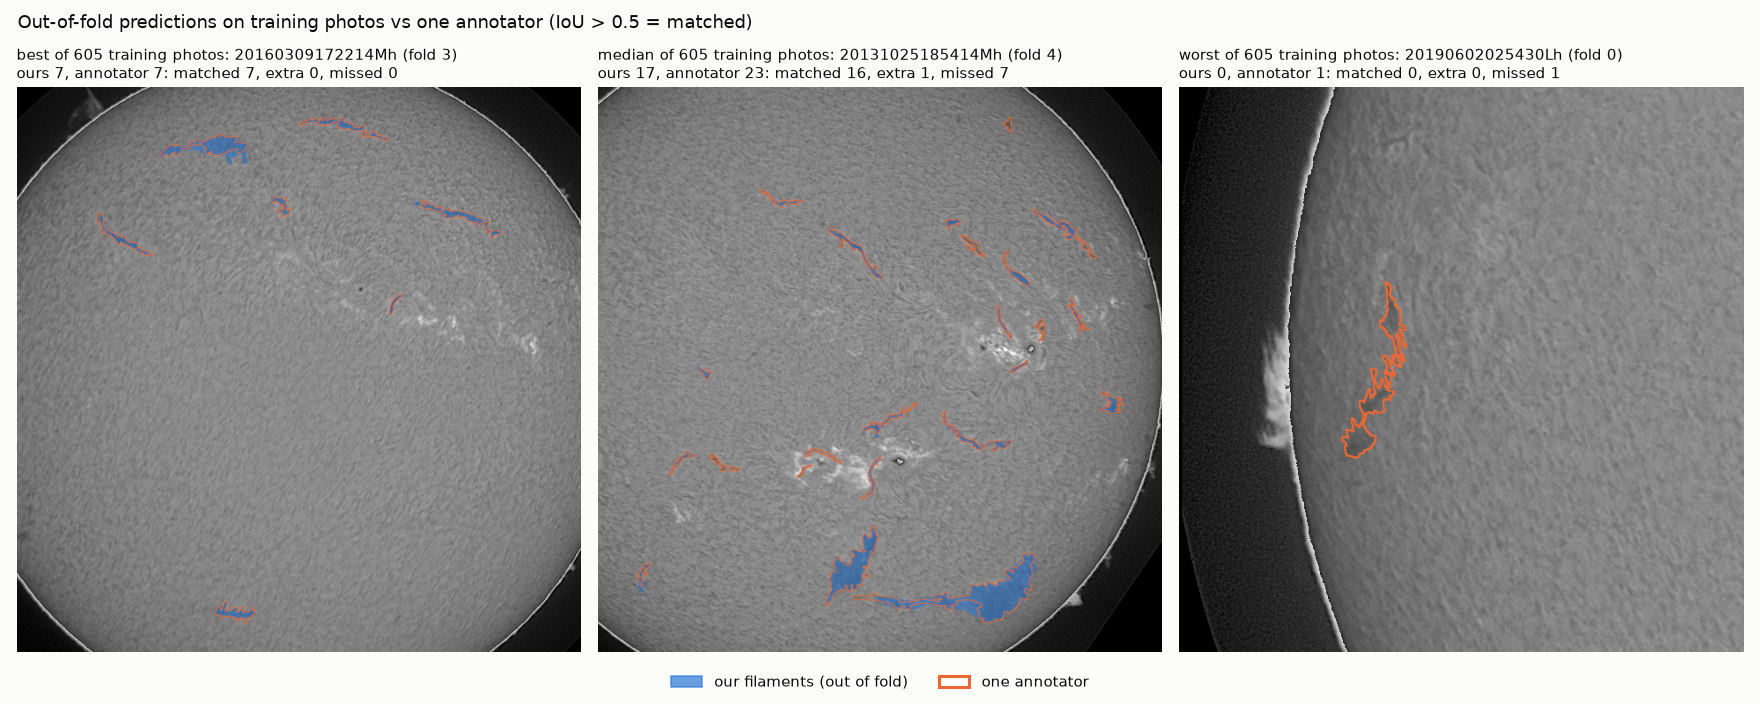
\includegraphics[width=\textwidth]{figures/oof_predictions.png}
\caption{Out-of-fold predictions of the final pipeline (filled blue) and one annotator's filaments (orange outlines) on three training observations, each predicted by models and a scorer that never saw it: the best, the median and the worst observation by match rate (observations with at least 4 annotated filaments).}
\label{fig:examples}
\Description{Three crops of solar disk images with predicted filaments filled in blue and one annotator's filaments outlined in orange.}
\end{figure*}

\begin{figure}[t]
\centering
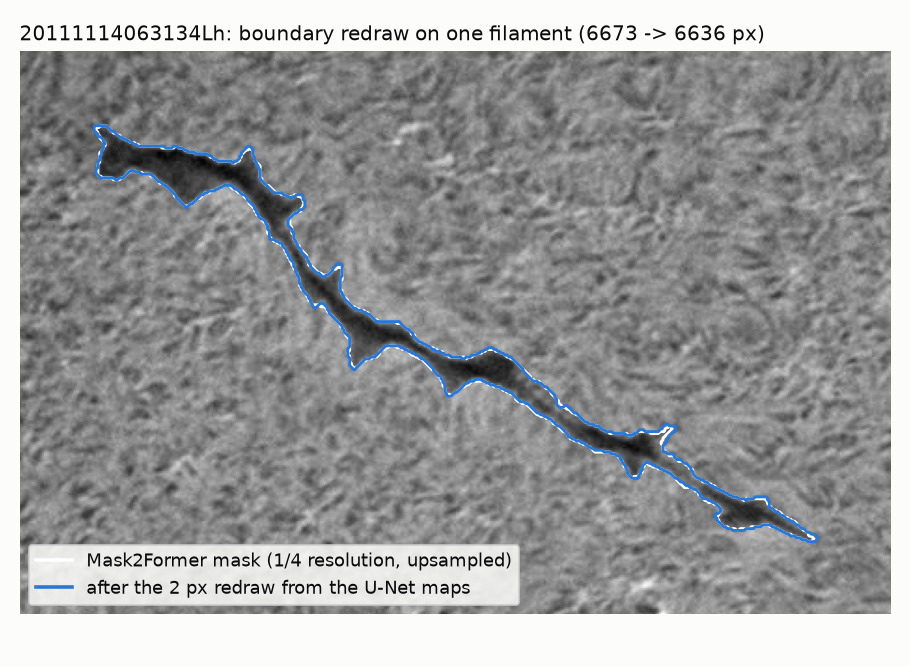
\includegraphics[width=0.78\columnwidth]{figures/redraw_closeup.png}
\caption{Boundary redraw on one test filament: the Mask2Former mask (white) and the mask after the 3-pixel redraw from the U-Net maps (blue).}
\label{fig:redraw}
\Description{Close-up of one filament with two outlines, white before and blue after the redraw.}
\end{figure}

\subsection{Strengths, weaknesses and possible improvements}
The main strength of the approach is that the submission decision is learned on the metric's own question, from evidence that is independent of the candidate generator, and solved exactly; every gain was measured out of fold with a paired interval. The whole pipeline is reproducible: a notebook downloads the data and the 40 trained models, checks their SHA-256, retrains any missing model, and rebuilds the submitted file byte for byte.

Its main weakness is the ceiling set by the annotations. Annotators agree with each other at a PQ of only 0.340. On observations with several annotators, 71\% of the OOF misses of our first model were filaments that no other annotator of the image drew, and 54\% of its false positives matched another annotator's filament. A scorer can only learn what the annotators have in common, which bounds what better selection can achieve. The pipeline is also heavy: 40 models and about 115 GPU-hours of training (about 28 hours on four 12\,GB GPUs), for gains of a few thousandths per step beyond the scorer.

Several ideas did not help out of fold and were not kept: filling gaps between candidates, merging split filaments, size-dependent thresholds, removing candidates near the limb, a larger scorer, contrast features, an HRNet evidence model, training with a centre-line (clDice) loss, a vote of scorers trained without each fold, and a convolutional scorer on candidate crops stacked into LightGBM ($-0.0010$). The most promising directions are therefore not more candidates but a better model of the annotators: training targets that represent each annotator's style, and a scorer that estimates the agreement between annotators rather than one consensus.


% ==================================== %
%            ACKNOWLEDGMENT            %
% ==================================== %
\section{Acknowledgment}\label{sec:acknowledgment}
    % Do not change
    The organization of the Filament Segmentation Challenge 2026 is partially supported by the U.S. National Science Foundation (NSF) under Grant No. 2209912 and 2433781, directorate for Computer and Information Science and Engineering (CSE), and Office of Advanced Cyberinfrastructure (OAC), and Grant No. 2511630, AST Division Of Astronomical Sciences and MPS Directorate for Mathematical and Physical Sciences.

    The Filament Segmentation Challenge 2026 is sponsored by the U.S. National Science Foundation (NSF) National Solar Observatory (NSO). 

    This work utilizes GONG data obtained by the NSO Integrated Synoptic Program, managed by the National Solar Observatory, which is operated by the Association of Universities for Research in Astronomy (AURA), Inc. under a cooperative agreement with the National Science Foundation and with contribution from the National Oceanic and Atmospheric Administration. The GONG network of instruments is hosted by the Big Bear Solar Observatory, High Altitude Observatory, Learmonth Solar Observatory, Udaipur Solar Observatory, Instituto de Astrofísica de Canarias, and Cerro Tololo Interamerican Observatory.

\bibliographystyle{ACM-Reference-Format}
\bibliography{main}

\end{document}
